\PassOptionsToPackage{dvipsnames}{xcolor}
\documentclass[border=0mm]{standalone}
\usepackage[dvipsnames]{xcolor}
\usepackage{amsmath}
\usepackage{amssymb}
\usepackage{dsfont}
\usepackage{bm}
\usepackage{tikz}
\usetikzlibrary{arrows}
\usetikzlibrary{calc}
\usetikzlibrary{shapes}
\usepackage{upgreek}

\usepackage{esvect}
\newcommand{\cev}[1]{\reflectbox{\ensuremath{\vv{\reflectbox{\ensuremath{#1}}}}}}


\definecolor{color1}{rgb}{0,0.4470,0.7410}
\definecolor{color2}{rgb}{0.8500,0.3250,0.0980}
\definecolor{color3}{rgb}{0.9290,0.6940,0.1250}
\definecolor{color4}{rgb}{0.4940,0.1840,0.5560}
\definecolor{color5}{rgb}{0.4660,0.6740,0.1880}
\definecolor{lightblue}{RGB}{86,192,150}

\pgfdeclarelayer{background layer}
\pgfdeclarelayer{foreground layer}
\pgfsetlayers{background layer,main,foreground layer}


\begin{document}



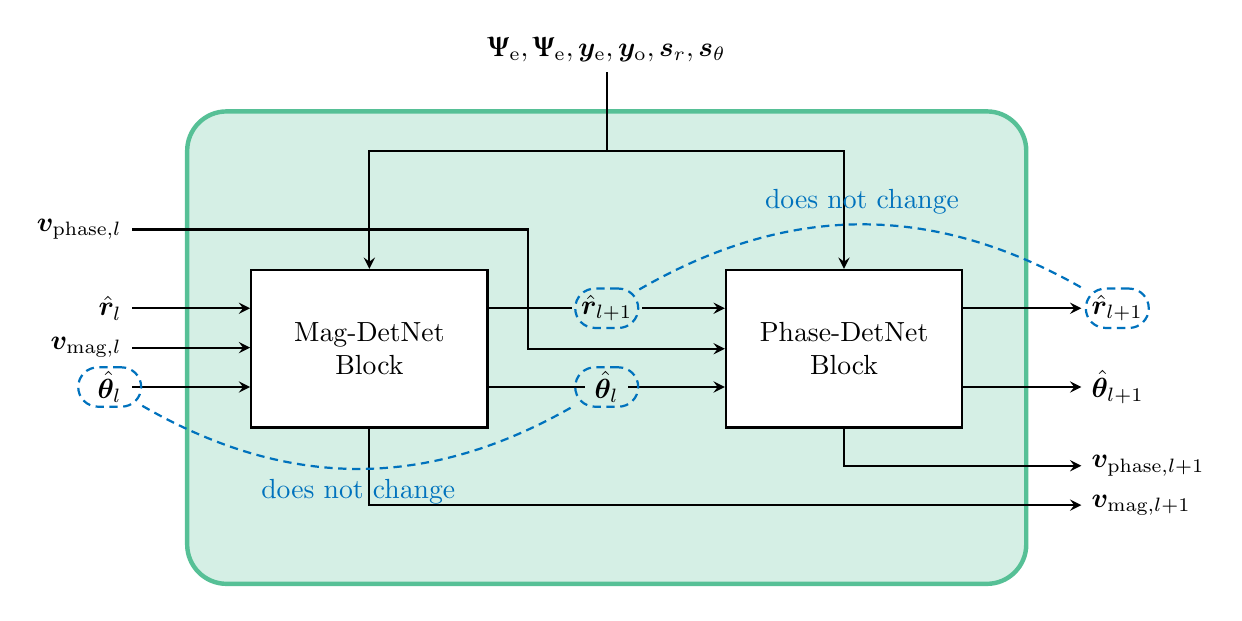
\begin{tikzpicture}[>=stealth,thick]

\node [fill=white,rectangle, draw, text width = 2cm, align=center, minimum width = 3cm, minimum height = 2cm, anchor=west] (magDetNet) at (0,0) {Mag-DetNet Block};

\node [fill=white,rectangle, draw, text width = 2.5cm, align=center, minimum width = 3cm, minimum height = 2cm, anchor=west] (phaseDetNet) at ($(magDetNet.east)+(3,0)$) {Phase-DetNet\\ Block};

\node [anchor=east] (r1) at ($(magDetNet.north west)+(-1.5,-0.5)$) {$\hat{\bm r}_l$};
\node [anchor=east] (vmag1) at ($(magDetNet.north west)+(-1.5,-1)$) {$\bm v_{\text{mag},l}$};
\node [anchor=east] (theta1) at ($(magDetNet.north west)+(-1.5,-1.5)$) {$\hat{\bm\theta}_l$};
\node [anchor=east] (vphase1) at ($(magDetNet.north west)+(-1.5,0.5)$) {$\bm v_{\text{phase},l}$};


\draw [->] (r1) -- (r1-| magDetNet.west);
\draw [->] (vmag1) -- (vmag1-| magDetNet.west);
\draw [->] (theta1) -- (theta1-| magDetNet.west);


\draw [->] (r1 -| magDetNet.east) -- node[midway, fill=lightblue!25](r2) {$\hat{\bm r}_{l+1}$} (r1 -| phaseDetNet.west);
\draw [->] (vphase1) -| ($(magDetNet.east)+(0.5,0)$) -- (phaseDetNet.west);
\draw [->] (theta1 -| magDetNet.east) -- node[midway, fill=lightblue!25] (theta2){$\hat{\bm \theta}_{l}$} (theta1 -| phaseDetNet.west);


\node [anchor=west] (r3) at ($(phaseDetNet.north east)+(1.5,-0.5)$) {$\hat{\bm r}_{l+1}$};
\node [anchor=west] (theta3) at ($(phaseDetNet.north east)+(1.5,-1.5)$) {$\hat{\bm\theta}_{l+1}$};
\node [anchor=west] (vphase3) at ($(phaseDetNet.north east)+(1.5,-2.5)$) {$\bm v_{\text{phase},l+1}$};
\node [anchor=west] (vmag3) at ($(phaseDetNet.north east)+(1.5,-3)$) {$\bm v_{\text{mag},l+1}$};

\draw [->] (phaseDetNet.east |- r3) -- (r3);
\draw [->] (phaseDetNet.east |- theta3) -- (theta3);
\draw [->] (phaseDetNet.south) |- (vphase3);
\draw [->] (magDetNet.south) |- (vmag3);

\node [anchor=south] (com1) at ($(r2)+(0,3)$) {$\bm{\Uppsi}_\text{e},\bm{\Uppsi}_\text{e},\bm y_\text{e},\bm y_\text{o},\bm s_r,\bm s_\theta$};

\draw [->] (com1.south) --+ (0,-1) node (com2){} -| (magDetNet.north);
\draw [->] (com2.center) -| (phaseDetNet.north);

\node [densely dashed,draw=color1,rounded corners=0.25cm,minimum width = 0.8cm, minimum height = 0.5cm] (e1) at (theta1){};
\node [densely dashed,draw=color1,rounded corners=0.25cm,minimum width = 0.8cm, minimum height = 0.5cm] (e2) at (theta2){};
\draw [densely dashed, color1] (e1) edge [bend right] node[below] {does not change} (e2);

\node [densely dashed,draw=color1,rounded corners=0.25cm,minimum width = 0.8cm, minimum height = 0.5cm] (e3) at (r2){};
\node [densely dashed,draw=color1,rounded corners=0.25cm,minimum width = 0.8cm, minimum height = 0.5cm] (e4) at (r3){};
\draw [densely dashed, color1] (e3) edge [bend left] node[above] {does not change} (e4);

\begin{pgfonlayer}{background layer}

\node (rec1) at ($(r1.east)+(0.7,0)$) {};
\node (rec2) at ($(r3.west)+(-0.7,0)$) {};
\node (rec3) at ($(com1.south)+(0,-0.5)$) {};
\node (rec4) at ($(vmag3)+(-5,-1)$) {};

\draw [ultra thick,draw = lightblue, fill=lightblue!25, rounded corners=0.5cm] (rec1 |- rec3) rectangle (rec2 |- rec4);

\end{pgfonlayer}

\end{tikzpicture}

\end{document}
























